\documentclass[11pt]{article}
\usepackage{graphicx}
\graphicspath{ {C:/Users/yedkk/Desktop/CS465/HW1} }
\begin{document}
\section{Homework 1}
Name: Kangdong Yuan

\subsection{probelm1}
a).I did not work in a group.
\\b).I did not consult without anyone my group members
\\c).I did not consult any non-class materials.
\subsection{probelm2}
a).
$R(0)=1,  \  R(1)=2, \ R(2)=3
\\R(i)=R(i-1)+R(i-2)+R(i-3) \ for \ i\geq2$

we want to prove that the $R(i)\geq 3^(\frac{i}{2}), \ for \ i \geq2$

begin with base case, for $i \ \geq 2$
\\$R(2)=3\geq3^1, \ R(3)=R(0)+R(1)+R(2)=6 \geq 3^\frac{3}{2}=5.19, \ R(4)=R(1)+R(2)+R(3)=11 \geq 3^2=9 $
\\
\\now, we assume that this claim holds for all case that $n<i+3 \ and \ i\geq2 $
\\$R_i=R_{i-1}+R_{i-2}+R_{i-3}=3^{0.5(i-1)}+3^{0.5(i-2)}=3^{0.5i}(\frac{1}{\sqrt{3}}+\frac{1}{3}+\frac{1}{3^{1.5}})\approx1.10313(3^{0.5i})\geq3^{\frac{1}{2}i}$
\\So $R(i)=R(i-1)+R(i-2)+R(i-3) \ for \ i\geq$
\\b).draw the recursive tree of R(i), take $R(7)$ as a example. 

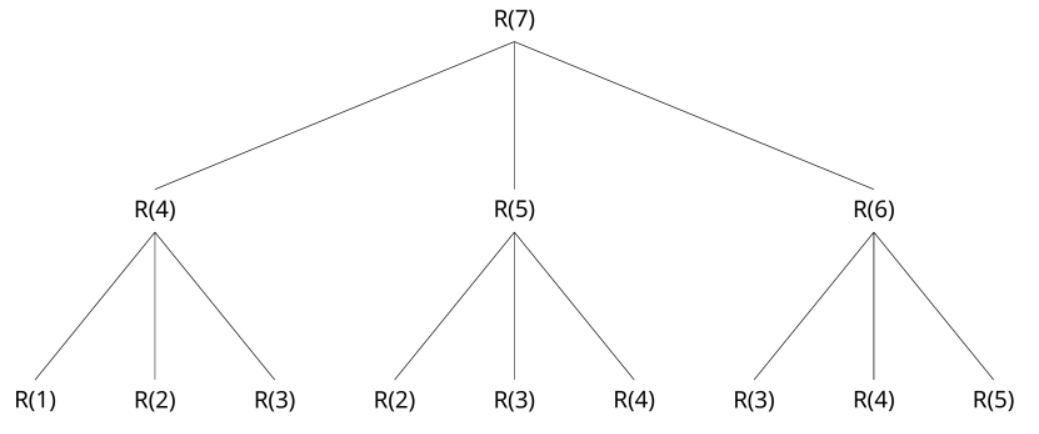
\includegraphics[scale=0.5]{Capture}

the one recursive call will triggered three another recursive calls, then three recursive calls will triggered another nine recursive calls. So the number of call in this recursive program are grow at exponential time.
\subsection{problem3}
we want to prove that $O_1(g(n))$ and $O_2(g(n))$ are equal. So, we want to prove that $c_1g(n_1)=c_2g(n_2)$ for $n_0> 0, \ n_1\geq n_0, n_2> 0$
\\we can prove that $n_1\geq n_0>0,  \ n_1>0$, so $n_1=n_2>0$
\\Because, $f(n)\leq c_1g(n_1), \ f(n) \leq c_2g(n_2) \ and \ n_1=n_2>0$, there must exist a $c=c_1=c_2$. So that $c_1g(n_1)=c_2g(n_2)$. when $n_1=n_2, \ c_1=c_2$. Thus $O_1(g(n))$ and $O_2(g(n))$ are equal, and the  two definitions are equivalent.
 

\subsection{Problem4}
1. the outer perform n times, and the inner loop take $i-1$ times. $\sum _{i=1}^n\:i=\frac{(n)(n+1)}{2}=O(n^2)$
\\The running time is $O(n^2)$
\\2. The outer perform n times. $i\leq\frac{n}{4}$, the j iterates $n-4i$ times. $\sum _{i=1}^{\frac{n}{4}}\left(n-4i\right)+\frac{3n}{4}\:=\frac{5n^2-8n}{16}=O(n^2)$ 
\\The running time is $O(n^2)$
\\3.We first try to explore the running time of outer loop.
\\When $i=n$, in each iteration $i/2$, after k iteration $\frac{n}{2^k}$, we get $k\leq log_2n$. The running time in outer loop is $O(log_2 n)$, the step in each inner loop is $i$. \\$\sum _{i=1}^{\log _2\left(n\right)}\:i=\frac{1}{2}\log _2\left(n\right)\left(\log _2\left(n\right)+1\right)=\frac{1}{2}(log_2nlog_2n+log_2n)=O(\log n \log n)$
\\4. the running time of outer loop is $O(n)$, the inner loop for $i\leq \sqrt{n}$, the j iterates $n-i^2$ times. 
\\$\sum _{i=1}^{\sqrt{n}}\left(n-i^2\right)+\left(n-\sqrt{n}\right)\:=\frac{5}{3}n\sqrt{n}-\frac{3}{2}n-\frac{1}{6}\sqrt{n}=O(n^{\frac{3}{2}})$
\\The running time is $O(n^{\frac{3}{2}})$

\subsection{problem5}
it seems this algorithm will take $O(n2^n)$ times, if we assume the bit flips in each iteration will increase and  the bit flips in each iteration is related to n.
But we calculate the steps of bit-flips of each iteration.
\\step5: 1(bit-flips), \\ step6: 2, \\ step7: 1, \\ step8: 4, \\step9: 1, \\step10:2, \\step11:1 \\...... \\step16:5, \\step17: 1 \\step30: 2, \\step31: 1
\\from our observation, the bit-flips in each iteration is the constant C that not related to n and $C\leq n$, the total running time is $\sum _{i=1}^{2^n}\:c=c*2^n=O(2^n)$. So it actually take $O(2^n)$
\end{document}